\chapterimage{chapter_head/3_429hero.jpg} 
%!TEX root = ../main.tex
\chapter{Applications to Intelligent Tutoring Systems}
\label{ch:its}
\vspace{-2.5cm}
\emph{Là-haut, le Château, déjà étrangement sombre, que K. avait
espéré atteindre dans la journée, recommençait à s’éloigner.
Mais, comme pour saluer K., à l’occasion de ce provisoire adieu,
le Château fit retentir un son de cloche, un son ailé, un son
joyeux, qui faisait trembler l’âme un instant : on eût dit – car il
avait aussi un accent douloureux – qu’il vous menaçait de
l’accomplissement des choses que votre cœur souhaitait obscurément. }\\ \vspace{-1.2cm}
\begin{flushright}\emph{Franz Kafka,} Le Château, \emph{Chapitre Premier}.
\end{flushright}
\blfootnote{Chapter header: \emph{À la croisée des mondes (Le Miroir d'ambre)}, John Howe, 2002. (Droits réservés)}
\section{Shortcomings in the bandits model}
\label{sec:shortcomings}
When we ask a question to a student, we observe their answer to this particular question. This is a good example of \emph{bandits feedback}. Facing this partial feedback, the machine learner has to explore the different options to understand what to do. Handling this exploration is the main question of the bandits' literature. This is quite relevant for adaptive Intelligent Tutoring Systems (ITS): if we think that different students should have different learning paths, we have to characterize to which extends a student is different. 

Of course, a good \emph{exploration} strategy depends on what we want to achieve. In the previous section, we have presented the most famous objective, \ie the cumulative reward maximization. The main objective is to balance between gathering new information and using this information to collect rewards. This exploration-exploitation dilemma is relevant for ITS: characterizing the student is only a tool to improve the learning. A good ITS should size the effort spent on characterizing the student versus the estimated benefits of such characterization. 

Yet, the cumulative reward maximization makes strong assumptions about the benefits. These assumptions strongly orientate the answers the bandits' community gives to this exploration-exploitation dilemma.
In the following, we will discuss four limits of applying classical bandits methods to Intelligent Tutoring Systems.

\subsection{Observation is reward.}
\label{ss:shortcoming-reward}
In the cumulative reward maximization setup, there is an identification between observation and reward. For an ITS, it is rather unclear what is the reward that can be associated with the student answer. One should be careful: the reward measures how well the ITS behaves and not how well the student answers the question. If we reward the ITS for the success of the student, the ITS will find very easy questions for the students, which is arguably not the best pedagogical strategy. In Section~\ref{sec:bandits4ITS}, we will present different rewards that were used for ITS applications. 

We advertise some objectives in the bandits' literature that are different from cumulative reward maximization. The Best Arm Identification (BAI) \citep{audibert2010bai, gabillon2012bai} is a pure exploration objective where the learner should output the best arm at the end of the game. There are several quantitative objectives associated with the best arm identification. In the fixed budget setting, one may want to minimize the \emph{simple regret} \citep{audibert2010bai}, that is, the difference between the true best arm's and the identified arm's values. Another possibility is to target the probability of outputting the best arm \citep{carpentier2016tight}. In the fixed confidence setting \citep{garivier2016optimalbai, kaufmann2016complexity}, the learner outputs as fast as possible with high-probability $1- \delta$ an arm at a residual distance $\epsilon$ from the best arm. The algorithms designed for cumulative regret do not work very well in the BAI setting. Indeed, at least from the asymptotical perspective, these algorithms spend $\cO\pa{\log{T}}$ in exploration and most of their budget in exploiting the identified best arm. 

The Best Arm Identification still considers observation as "reward", in the sense that the motivation of targeting the arm with the largest observation is based on the identification "large observation = good". This is not the case for Thresholding Bandits \citep{locatelli2016thresholding, garivier2016thresholding, mukherjee2017thresholding} where the learner wants to separate the arms according to their position relative to a threshold. Interestingly, \citet{locatelli2016thresholding} found a near-optimal algorithm which is fully agnostic. This problem is interesting from an educational perspective: if we have several topics with corresponding sets of related questions, we may want to know which topics are mastered by a student. We could define a threshold above which the topic is considered as mastered and use a Thresholding Bandits algorithm.

More generally, \emph{exploration} can be intrinsically interesting for ITS if the goal is to send information to the teacher. That is why \citet{liu2014trading, erraqabi2017trading} considered a setup where the objective combines the cumulative reward and the error the learner do on the estimation of each arm. \citet{erraqabi2017trading} show that naive \UCB algorithm fails in this setting. They describe \ForcingBalance, an algorithm that directly targets the optimal allocation of pulls for this problem. 


\subsection{Comparing to the best action.}
\label{ss:shortcoming-oracle}
In both the stationary and the adversarial setups, the performance is compared with the policy which selects always the "best" action. For ITS applications, we believe that the best thing to do is not to recommend always the same type of exercises. 

In Sections~\ref{sec:non-stationary} and~\ref{sec:contextual}, we presented two lines of work where the optimal action is not always the same during the game. These approaches have some limits. Contextual bandits need a meaningful representation for the context such that the reward is a simple function in this space. This representation can be learned using offline data, but it breaks the online paradigm. Moreover, contextual algorithms often use more sophisticated techniques. For instance, the simple averages which are used in the classical multi-armed bandits' framework (e.g., for computing the ucb) are replaced by regression methods which are computationally more expensive. Non-stationary bandits also have some important drawbacks. They often require much more exploration than in the stationary case. This is especially true in the restless case, when arms which are not pulled can change. Indeed, this type of non-stationarity is particularly challenging with bandit feedback. 

\subsection{Actions do not impact observations}
\label{ss:shortcoming-non-stationary}
In the classical adversarial and stochastic setting, the learner has no impact on the observations (rewards) output by the arms. This is a strong limitation for tutoring systems, as we expect a teaching strategy to modify the student's knowledge. 

Reinforcement Learning (Section~\ref{sec:rl}) models a more general setup where the learner has a state which is changed by the action. In some non-stationary bandits setups (Section~\ref{sec:non-stationary}), arms reward is changing when the arm is pulled. It could be reformulated as a "state" which is impacted by the actions of the learner. There is a difference of perspective between RL and non-stationary bandits: bandits methods often focus on tracking the changing rewards to target the (often short-sighted) best action while RL methods design policies that monitor the state's dynamics to remain in rewarding regions of the state space. 

\subsection{Learning is quite slow.}
\label{ss:shortcoming-slow}
The last paragraphs suggest increasing the complexity of the classical bandits model with context, state, or non-stationarity. However, the stationary stochastic bandits are already quite hard to learn when the horizon is small. Indeed, students often do no more than a few tens (or hundreds) questions. By contrast, bandits algorithm are often evaluated for longer horizon $T > 10^4$ (e.g., \citet{chapelle2011empirical}). 

From the theoretical perspective, the asymptotic rate $\cO\pa{\nicefrac{\log T}{\Delta_i}}$ is larger than the maximal regret $T\Delta_i$ for many gaps $\Delta_i < 0.2$ when the horizon is small ($T=100$). It means that the asymptotic analysis is not meant for such small horizons (except when the gap is very large). Even the minimax rate $\cO\pa{\sqrt{KT}}$ is not very different from the worst possible rate $T$ for small $T$.

This \emph{small data} situation is particularly challenging. Special care should be taken to overcome this issue: The learning problem should not be too ambitious, the setup should be correctly designed. In particular, the number of arms (or unknown reward parameters for contextual bandits) should be reduced. Prior information should be included in the model, algorithms should target finite-time and empirical performance.

\section{Exploration methods in Adaptive Intelligent Tutoring Systems}
\label{sec:bandits4ITS}

In this section, we will review previous work which involves bandits and reinforcement learning methods in Intelligent Tutoring Systems.  We will focus on the work where the action-observation loop corresponds to the sequence of question-answer of a single student. In these setups, the goal is to explore the student's knowledge and exploit this knowledge to improve educational actions.

Notice that there are also different exploration scenarios where the feedback loop is the sequence of incoming students. The goal is to refine the instructional policy from one student to another. The objective can be to choose the courses that maximize the final grade of the student \citep{xu2016personalized, lan2016contextual}, or to find the teaching examples sequence that maximizes the score at the test \citep{lindsey2013optimizing}.

\subsection{Target the largest improvement}
\citet{clement2015multi} suggest an ITS which selects sequentially a question linked to a knowledge component (KC) and receives the answer of the student. They suggest selecting the action which leads to the largest increase in student's performance. Besides maximizing the learning gain, it is also the action that motivates the most the learner \citep{gottlieb2013information}. 

\begin{figure}[h]
\begin{center}
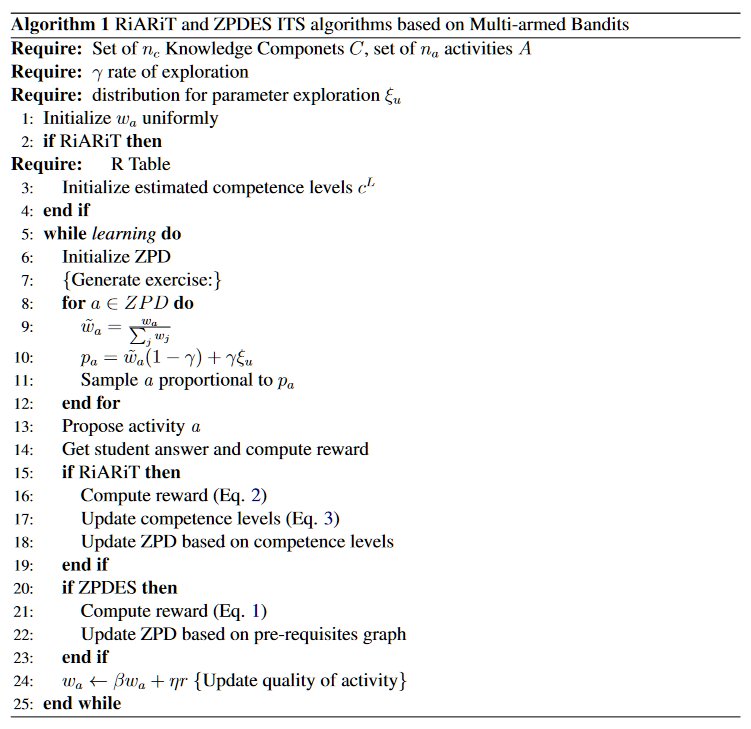
\includegraphics[scale=1]{fig/2Litterature_uncompressed/lopes-alg.png}
\end{center}
\caption{\citet{clement2015multi}'s algorithms}
\label{alg:clement}
\end{figure}

They present two similar algorithms which we reproduce in Figure~\ref{alg:clement}. Each algorithm has two components: the first one computes a \emph{Zone of Proximal Developement} (ZPD, \citet{luckin2001designing}), the second selects one knowledge component in the ZPD. The ZPD aims to exclude the KCs on which the student is either too good, too bad, or the ones on which s/he does not progress.  These algorithms don't use any model nor parametric assumption on the way the student progresses. They compute non-parametric statistics to estimate the current level or the current progress of the student on a KC.

Once the ZPD is set, a bandit algorithm selects a KC. The reward is a difference between the last samples and the before last ones. In the first algorithm (Zone of Proximal Development and Empirical Success - \ZPDES), they use the average of the $\nicefrac{d}{2}$ last samples minus the average $\nicefrac{d}{2}$ before last samples. In the second algorithm (Right Activity at the Right Time - \RiARiT), they use the last sample minus a discounted average of the previous ones. These two statistics measure the recent progress of the students. 

They claim to use a variant of \EXPfour \citep{auer2002nonstochastic}. Like \EXPfour, this algorithm is probabilistic (see Line~11 in Fig.~\ref{alg:clement}). The output probability distribution pulls arm according to weights, which are a weighted sum of rewards. This probability distribution also has a uniform component $\xi_u$, like the vanilla \EXPfour. Notice that this component was later proven to be unnecessary \citep{bubeck2012regret}, even to recover high probability guarantees \citep{neu2015explore}. 

Yet, this bandit algorithm also has major differences with \EXPfour. First, there are no experts recommendations which are a necessary input of \EXPfour. Hence, this algorithm is closer to \EXP. In Subsection~\ref{sec:adv-bandits}, we presented the three ideas beyond \EXP: Follow the regularized leader, a specific regularization, and an unbiased estimation scheme based on importance weight. The specific regularization is responsible for the exponential weights, which are absent from the algorithm of \citet{clement2015multi}. The importance weights of the loss -  the loss is divided by the probability of pulling the arm - are replaced by fixed weights $\beta$ and $\nu$ on the reward (see Line~24). These fixed weights are closer to discounted statistics used in non-stationary bandits (like \DUCB, \citet{kocsis2006discounted, garivier2011upper-confidence-bound}). 

Anyway, the main feature of \EXP is to guarantee $\tcO\pa{\sqrt{KT}}$ regret compared to the sum of the reward for the policies which select always the same arm. In this setup, we believe that the interest of this result is limited for two reasons. First, the policies which selects always the same KCs are not the most interesting policies from the educational point of view. Second, the rewards are weighted differences of past observations. Hence, there is a telescoping effect in the cumulative reward. For some choices of parameters in the reward definition (e.g. $d=2$ for \ZPDES), this telescoping can be total such that the sum of the rewards is simply the last observation minus the first, \ie a $\cO\pa{1}$ quantity. In that case, the $\tcO\pa{\sqrt{KT}}$ guarantee is meaningless. Even for other choices of parameters, the telescoping reduces the cumulative reward range. The more that range is reduced \emph{by construction}, the less interesting is the theoretical guarantee of \EXP.

Hence, we believe that the modifications suggested by \citet{clement2015multi} are indeed more interesting than the classical \EXP. Their algorithm targets a more pragmatic goal: selecting randomly the KCs (to ensure diversity in the tasks) while favoring smoothly the KCs which demonstrate recent progress. They provide empirical evidence of the benefits of their algorithms. In a simulated experiment, they show that their algorithms are more adaptable than an expert sequence to the profile of some simulated students. In an in-class experiment on real students, they show that students who were learning with their algorithms achieve more balanced performance between KCs than a control group that was using the expert sequence. They also demonstrate qualitative differences between the behavior of their algorithm and the expert sequence. 

As noticed by \citet{pikeburke2019phd}, this paper is arguably one of the most advanced works using bandits in ITS. The objective - targeting the topic on which the student progresses - is very appealing. The ZPD design allows some timely exploration by unlocking progressively the most advanced topics. The experiments bring many insightful comparisons between the studied algorithms and the expert sequence. However, this work only partially address the aforementioned shortcomings~\ref{ss:shortcoming-oracle}, \ref{ss:shortcoming-non-stationary}, and~\ref{ss:shortcoming-slow}.

In particular, there are statistical issues with respect to shortcomings~\ref{ss:shortcoming-oracle} and~\ref{ss:shortcoming-non-stationary}. The goal of the paper is to aim at the arm with the current largest increase. It is not clear that this problem fall under the cumulative reward maximisation perspective (see our discussion on the telescoping effect). Even in the algorithm, it is not clear that taking a discounted sum of rewards, which are themselves differences of past observations is a statistically efficient way to measure recent progress. We also notice that these algorithms are quite difficult to tune. They have 4 parameters: $\gamma$, $\nu$, $\beta$ and an other parameter for the reward computation.

The work of \citet{clement2015multi} was further extended by \citet{mu2018combining} to take into account the forgetting of the student and the learning of the ZPD structure. 

We also advertise the works of \citet{rollinson2015predictive, kaser2016stop}, which also try to track the progress of the student. These works do not aim at choosing the knowledge component among several possibilities. Instead, they try to decide when one should stop the work on a given skill. \citet{rollinson2015predictive} suggest stopping when there is a sufficient probability that the prospective learning gain associated with the next question is below a threshold. The prospective learning gains are estimated with a student model. Notice that these models are trained with the data of many other students such as it reflects the "average" student.  The models assume a specific shape of the progression. Hence, different models with the same input sequence can lead to different stopping times, even when they have comparable predictive performance. The issue is that the predictive performance is evaluated on several students, the goal is to predict correctly on average. However, when they are used in instructional policies, these models are required to explain and predict quantitatively the learning of a specific student given a small amount of data. This instructional policy was further extended by \citet{kaser2016stop} to be able to stop when a student's performance diverges from the model (for instance, for wheel-spinning student) and to include more complex student models such as deep belief network. 

\subsection{Target the least known subject}
\label{ss:less-known}
\citet{melesko2019computer} suggest targeting the less known subjects. The idea is that the student has more to learn from their mistakes than from their successes. Hence, they suggest rewarding the failed questions and to not reward the succeeded ones. 

Rewarding the system for finding the failed exercises has some limits. Some skills are harder to get, and it could be useful to start with the simplest one. It can also be the case that there are some prerequisite dependencies between the different skills. From the motivational point of view, recommending too hard questions may disengage the student. 

Yet, consider a student that is learning some geography facts. S/he wants to check if s/he know their lesson. The different topics in the lesson are as hard to learn \emph{a priori}. Yet, the student could have studied a lot the first part of the course and did not spend too much effort on the other parts. The goal of the ITS could be to try to spot the weaker part of the course and teach them with some questions.

Another motivation highlighted by \citet{melesko2019computer} is the pure-exploration setup, where the goal of the ITS is to find the weakest topic to send the information to the teacher. 

\citet{melesko2019computer} suggest using the classical \UCB algorithm. They carry many very small data experiments where the number of topics (arms of the bandits) is of the same order of magnitude as the number of questions (horizon). In this context, they recommend the usage of smaller confidence intervals than classical \UCB. The experiments show improved performance for \UCB compared to the random strategy. 

In their work, \citet{melesko2019computer} neglect the impact of the questions on the knowledge of the student. The goal is not really to teach through questions, but to find the least understood topic. However, it is surprising that they use an exploration-exploitation algorithm instead of a specialized algorithm from the best arm identification literature. 

\citet{teng2018interactive} also target to find the least known questions with multi-armed bandits methods. They suggest an algorithm adapted from the linear bandits' literature where the reward depends linearly on an embedding. The algorithm uses several graphs structuring questions, users, and concepts. These graphs are used to infer a vector representation of the users and questions. They bring theoretical and empirical evidence of the performance of their algorithm. 

\subsection{Target faster learning}
\citet{rafferty2016faster} suggest minimizing the time the student spends to understand a concept. Hence, the cost (negative reward) associated with each pedagogical action is the time the action takes to be completed. They formulate their problem as a Partially Observable Markov Decision Process. Indeed, the student has a knowledge state which is only partially observable by the teacher. The teacher has several actions: some \emph{examples} which teaches the concept to the student, some \emph{quizzes} which retrieves information about the knowledge state of the student, and some \emph{questions with feedback} which do both at the same time.  The goal of the learner is to track the state of the student (which encodes what the student does not know) with questions to show some relevant examples. 

They test this framework with several student models and several learning scenarios. The algorithm shows significant time reduction compared to random policies. Some student models are better than others. In particular, modeling long-term memory improves performance compared to models that react only to the last seen example.